%% Informe en formato IEEE (IEEEtran) - Tarea 1 Aprendizaje Automatico 2026
%% Compilable en Overleaf con la plantilla IEEE Conference.
\documentclass[conference]{IEEEtran}
\IEEEoverridecommandlockouts
\usepackage{cite}
\usepackage{amsmath,amssymb,amsfonts}
\usepackage{graphicx}
\usepackage{booktabs}
\usepackage[spanish]{babel}
\usepackage[utf8]{inputenc}
\usepackage{url}
\usepackage{multirow}
\usepackage{xcolor}


\begin{document}

\title{Predicción de resultados del fútbol uruguayo mediante aprendizaje supervisado}

\author{\IEEEauthorblockN{Cecilia Waksman, Lucia Coudet}
\IEEEauthorblockA{\textit{Aprendizaje Automático 2026} \\
\textit{Facultad de Ingeniería, Udelar}\\
Montevideo, Uruguay}}

\maketitle

\begin{abstract}
Se aborda la predicción del resultado de partidos del fútbol uruguayo según gane el cuadro local, el cuadro visitante, o haya empate, a partir del conjunto de datos de David Schoch, restringido a los años 1932--2025. Se construye un pipeline reproducible de preprocesamiento y \emph{feature engineering} temporal y causal. Se
implementan un árbol de decisión con el hiperparámetro
\texttt{min\_info\_gain} y un clasificador Naive Bayes con m, tamaño equivalente de muestra. Asimismo, se implementa un clasificador base que prediga que gana el equipo que tiene mayor proporcion de partidos ganados en los últimos 10 años. Se
comparan los resultados obtenidos con los de Random Forest y Naive Bayes de scikit-learn. Como resultado se obtiene que \textcolor{red}{PONER RESULTADOS PARTE 2}. Luego se realiza un ajuste con técnicas de validación cruzada y ajuste de hiperparámetros y se compara el desempeño de todos los clasificadores implementados. Teniendo en cuenta las medidas de precisión, recall, F1 por clase, accuracy y macro F1 se concluye que \textcolor{red}{PONER CONCLUSION ACA}
\end{abstract}

\begin{IEEEkeywords}
aprendizaje supervisado, fútbol, árbol de decisión, Naive Bayes, series temporales
\end{IEEEkeywords}

\section{Introducción}
Predecir el resultado de un partido de fútbol es un problema clásico de
clasificación multiclase con tres salidas: gana el local (\texttt{L}), hay empate
(\texttt{E}) o gana el visitante (\texttt{V}). El fútbol posee una fuerte
componente aleatoria, por lo que incluso modelos informados rara vez superan de
forma amplia a heurísticas simples. En este trabajo se utiliza el conjunto de
datos público de resultados de ligas de David Schoch~\cite{schoch}, restringido
a los partidos del fútbol uruguayo entre 1932 y 2025 (15.207 registros).

Dicho conjunto contiene información sobre:
\begin{itemize}
	\item home: nombre del cuadro local
	\item away: nombre del cuadro visitante
	\item date: fecha del partido
	\item gh: número de goles del cuadro local
	\item ga: número de goles del cuadro visitante
	\item full time: indica si el partido terminó a los 90 minutos, si hubo tiempo extra, o si huvo penales
\end{itemize}

Asimismo, el conjunto de datos contiene información sobre el identificador, país, código, y continente del cuadro local y del cuadro visitante, y el continente donde se realizó la competición. 

Los objetivos son: (i) construir un pipeline reproducible de preprocesamiento;
(ii) implementar clasificadores supervisados, incluyendo dos algoritmos propios;
y (iii) evaluar el desempeño con un protocolo temporal riguroso que evite fugas de información, implementando técnicas de validación cruzada. 

\section{Preprocesamiento}

El preprocesamiento implementado consiste en la realización de la limpieza de los datos y de la transformación a un formato aceptable para los algorimos a utilizar.

En lo que respecta a la limpieza, se verifica que las columnas no tienen errores y que no hay valores faltantes en ningún atributo. Asimismo, se eliminan filas duplicadas. También se verifica que los años de las fechas de los partidos se encuentran dentro del rango esperado: 1932-2025.

En lo que respecta a la transformación de los datos, se definieron los tipos de atributos (numéricos, categóricos, fechas) y se eliminaron los atributos constantes que no aportan información al algoritmo (home country, away country, home code, away code, home continent, away continent, continent, level).

Para evitar la fuga de información (\textit{data leakage}), se elimina el atributo \textit{full time} ya que contiene información que no es posible conocer antes de que el partido termine. Introduce una correlación con el resultado del tiempo regular, ya que para que exista tiempo extra o panales es necesario que el resultado en tiempo regular haya sido empate. Incluir esta variable le otorga al algoritmo una pista directa del desarrollo del encuentro que invalida su capacidad predictiva real para futuros partidos. En la medida que es información que no se tiene a priori, no sería posible utilizar el modelo para predecir nuevos resultados si se mantuviera en el conjunto de entrenamiento.

En lo que respecta a la creación de nuevos atributos, se crearon a partir del atributo "fecha": el año, el mes, y el dia de la semana en el que se llevó a cabo el partido, y una variable indicatriz que indica si fue realizado un fin de semana.

También se creó el atributo "tasa de victorias local" y "tasa de victoria visitante" que indica la tasa de victorias del cuadro local y visitante respectivamente, considerando una ventana móvil de los últimos 5 años, y la diferencia entre ellas.

Finalmente se crea el atributo objetivo \texttt{resultado} comparando los goles de local y visitante y siendo los posibles resultados: gana el cuadro local, gana el cuadro visitante, o hay empate.

Una vez creados los nuevos atributos definidos anteriormente y realizada la limpieza mencionada, se realiza la transformación de los datos según tipo de columna:

\begin{itemize}
\item A las columans categóricas se le acplica one-hot encoding utilizando la función  OneHotEncoder de la libreria sklearn.preprocessing, para la implementación del árbol de decisión
\item A las columnas numéricas se las mantiene tal como estan, ya que se verifica que ambas pertenecen al intervalo 0-1 (no es necesario escalar)
\end{itemize}

\section{Modelos Supervisados}

\subsection{Partición de la muestra}

Para la implementación de los modelos de prendizaje supervisado, se realizó una partición de la muestra en conjunto de entrenamiento y conjunto de evaluación que considera la temporalidad de los datos, en particular en lo que respecta al orden cronológico de los mismos, de manera de asegurar que para realizar predicción en un determinado momento del tiempo se utilizó información disponible hasta ese momento del tiempo, evitando así la fuga de información (\textit{data leakage}). En particular, se consideraron los partidos jugados hasta el año 2023 como conjunto de entrenamiento y los jugados en 2024 y 2025 como conjunto de evaluación.

\subsection{Feature selection}

Se realiza la selección de los atributos más importantes calculando la información mutua (\textit{mutual information}) entre cada atributo del conjunto de datos y la variable objetivo, con el fin de rankear y seleccionar las características con mayor capacidad predictiva.

La información mutua intenta medir cuánta incertidumbre sobre la clase objetivo se reduce al conocer el valor de cada variable. Un valor de 0 indica independencia total mientrs que valores más altos reflejan una relación de dependencia más fuerte.

Para la codificación de las variables catgóricas se utiliza la función \textit{OrdinalEncoder} que transforma  las categorías en números enteros.

Se decide eliminar los atributos que aportan una ganancia de información inferior a 0.01. Los atributos eliminados son el que indica el día de la semana en que se jugó el partido y la variable indicatriz que indica si fue fin de semana.


\subsection{Árbol de decisión con parmámetro \texttt{min\_info\_gain} - Manual}

Para la implementación propia del árbol de decisión se implementa la técnica de one hot encoding en el preprocesamiento, de forma de convertir los atributos categóricos en nuevas columnas binarias.

Durante el entrenamiento, el algoritmo construye el árbol de forma recursiva dividiendo los datos en cada nodo según la variable y umbral que maximizan la ganancia de información (basada en la reducción de entropía). Maneja tanto variables numéricas como categóricas. El crecimiento se detiene al alcanzar hojas puras, una profundidad máxima, un número mínimo de muestras o cuando la ganancia cae por debajo de la ganancia mínima de información especificada, asignando en las hojas la clase mayoritaria. En la parte de predicción, se evaluan nuevas observaciones recorriendo la estructura desde la raíz hasta la hoja correspondiente para retornar la clase predicha.

A continuaciòn se presenta la matriz de confusión obtenida habiendo especificado en el algoritmo una ganancia de información mínima de 0.01:

\begin{figure}[htbp]
	\centering
	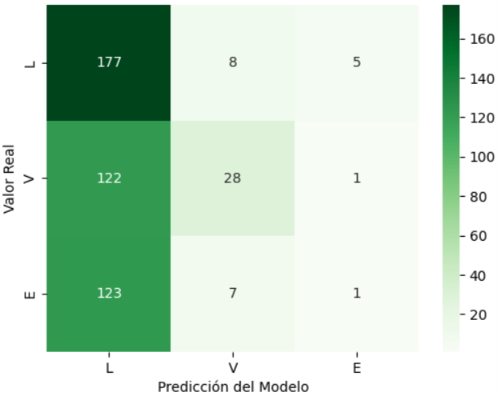
\includegraphics[width=0.3\textwidth]{graficos/cm_arbol_manual.png}
	\caption{Matriz de confusión del Árbol de Decisión manual}
	\label{fig:mi_grafico}
\end{figure}

\subsection{Árbol de decisión - Scikit Learn}

Se realizó la implementación del árbol de decisión mediante el clasificador de Scikit Learn \textit{DecisionTreeClassifier}, con los siguientes parámetros: \textit{min impurity decrease = 0.001}, \textit{max depth = None}, \textit{criterion = Entropy}, \textit{min samples leaf = 100}.

\begin{figure}[htbp]
	\centering
	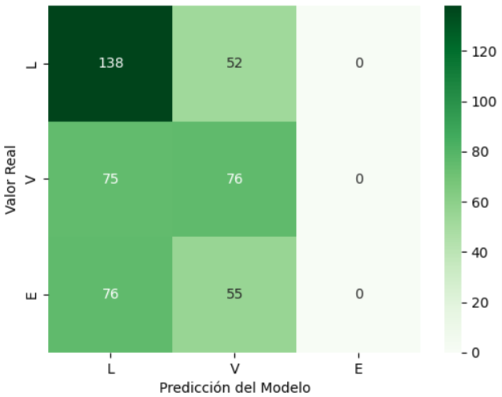
\includegraphics[width=0.3\textwidth]{graficos/cm_arbol_scikit.png}
	\caption{Matriz de confusión del Árbol de Decisión Scikit Learn}
	\label{fig:mi_grafico 1}
\end{figure}

Se verifica que la clase 2 "Hay empate" tiene precision y recall 0. Esto puede deberse a:

\begin{itemize}
	\item Desbalance severo de clases: La clase con 0 accuracy representa un porcentaje muy pequeño del conjunto de datos y el árbol la ignora para maximizar el accuracy global.
	\item El árbol está sobreajustado o simplificado en exceso
	\item Métrica de optimización incorrecta por utilizar el accuracy como criterio de optimización, el cual prioriza a las clases con más muestras.
\end{itemize}

Se propone balancear el peso de las clases utilizando el argumento \textit{class weight='balanced'}, esto le da más importancia (penalización) a los errores cometidos en las clases con menos muestras. A continuación se presenta la matriz de confusión obtenida en este ajuste:

\begin{figure}[htbp]
	\centering
	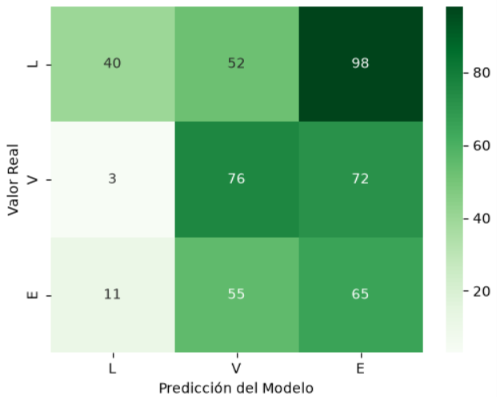
\includegraphics[width=0.3\textwidth]{graficos/cm_arbol_scikit2.png}
	\caption{Matriz de confusión del Árbol de Decisión Scikit Learn 2}
	\label{fig:mi_grafico 2}
\end{figure}

\subsection{Naive Bayes con parámetro $m$ - Manual}

Se implementa de manera manual un clasificador Naive Bayes Categórico compatible con Scikit-Learn. En el entrenamiento, calcula las probabilidades a priori de las clases y las condicionales utilizando el m-estimador para suavizar probabilidades de valores ausentes o sin frecuencia. En el predict, suma los logaritmos de estas probabilidades por fila para seleccionar la clase con mayor valor acumulado. Por último, entrena el modelo con parámetro m=1 y evalúa sus predicciones imprimiendo la métrica de Accuracy y el Classification Report.

A continuación se presenta la matriz de confusión obtenida:

\begin{figure}[htbp]
	\centering
	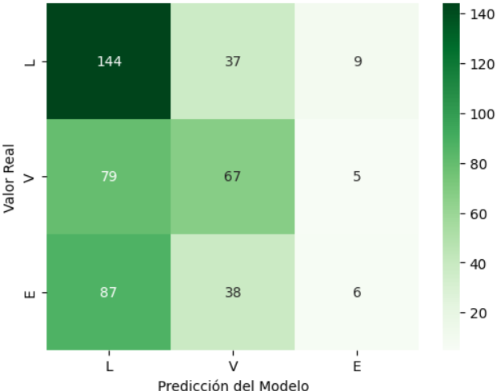
\includegraphics[width=0.3\textwidth]{graficos/cm_nb_manual.png}
	\caption{Matriz de confusión del ajuste Naive Bayes manual}
	\label{fig:mi_grafico 3}
\end{figure}

\subsection{Naive Bayes con parámetro $m$ - Scikit Learn}

También se implemento el ajuste utilizando el clasificador de la librería Scikit Learn \textit{CategoricalNB} con parámetros \textit{alpha=1} y \textit{fit prior = True}.

LA matriz de confusión obtenida fue la siguiente:

\begin{figure}[htbp]
	\centering
	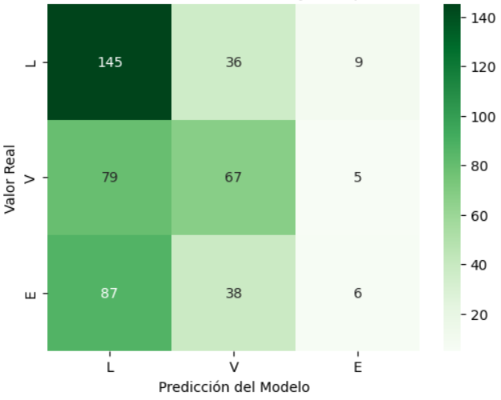
\includegraphics[width=0.3\textwidth]{graficos/cm_nb_scikit.png}
	\caption{Matriz de confusión del ajuste Naive Bayes Scikit Learn}
	\label{fig:mi_grafico 4}
\end{figure}


\subsection{Clasificador base}

Se implementó un clasificador base que en el entrenamient , identifica la clase mayoritaria global y calcula la tasa histórica de victorias de cada equipo considerando únicamente los últimos 10 años. En el predict, compara la tasa de victorias del equipo local contra el visitante: predice local (L) o visitante (V) según cuál tenga mayor tasa, y asigna la clase mayoritaria en caso de empate o falta de datos. Finalmente, ajusta el modelo con los datos de entrenamiento y evalúa sus predicciones en el conjunto de prueba imprimiendo Accuracy y Classification Report.

A continuación se presenta la matriz de confusión obtenida:

\begin{figure}[htbp]
	\centering
	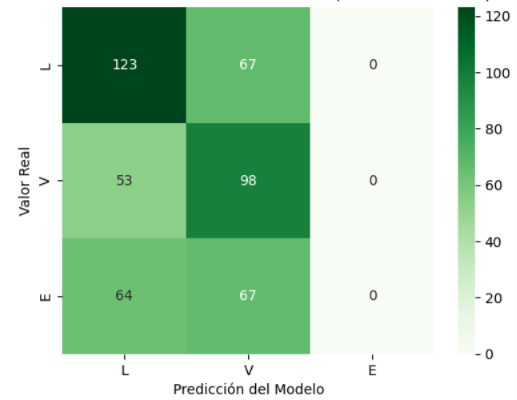
\includegraphics[width=0.3\textwidth]{graficos/cm_cb_manual.png}
	\caption{Matriz de confusión del ajuste Naive Bayes Scikit Learn}
	\label{fig:mi_grafico 5}
\end{figure}

\subsection{Random Forest - Scikit Learn}

Por último, se realizó un ajuste mediante el método de Random Forest utilizando el clasificador de Scikit Learn \textit{RanfomForestClassifier} con parámetros n estimators=300,
max depth=None, min samples leaf=10, max features="sqrt",
random state=42, n jobs=-1. 

Se obtuvo la siguiente matriz de confusión:

\begin{figure}[htbp]
	\centering
	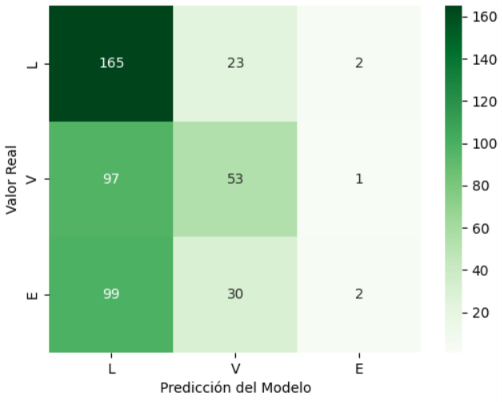
\includegraphics[width=0.3\textwidth]{graficos/cm_rf_scikit.png}
	\caption{Matriz de confusión del ajuste Naive Bayes Scikit Learn}
	\label{fig:mi_grafico 6}
\end{figure}

\subsection{Comparación de modelos}

A modo de resumen, se presenta el gráfico con el accuracy obtenido en cada uno de los métodos comentados en las subsecciones anteriores. Como puede observarse, el Clasificador Base es el que tiene un valor mayor para esta medida, mientras que el Árbol de Decisión de Scikit Learn el menor.

\begin{figure}[htbp]
	\centering
	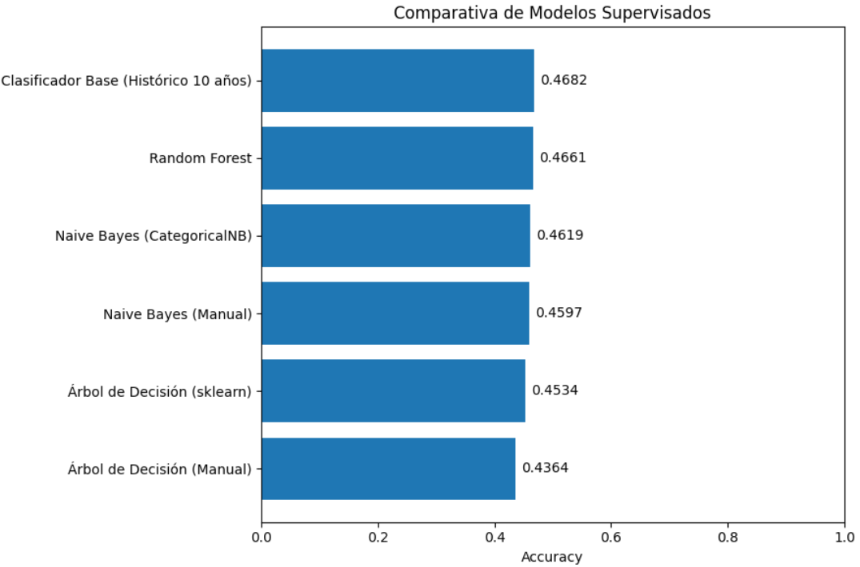
\includegraphics[width=0.5\textwidth]{graficos/comparacion_parte_2.png}
	\caption{Accuracy de los modelos ajustados}
	\label{fig:mi_grafico 7}
\end{figure}


\section{Experimentación}

En la etapa de experimentación, se definió un pipeline de preprocesamiento para cada modelo según los atributos a utilizar en cada algoritmo y las transformaciones específicas.

\subsection{Tratamiento de la temporalidad}

Sobre el conjunto de entrenamiento definido anteriormente, que contiene información de los partidos jugados hasta el año 2023 inclusive,  se definió función de validación cruzada con ventanas móviles de 1 año, las cuales definen los grupos utilizados para validar. Se definieron 5 grupos de 1 año cada uno usando los datos hasta 2019, y para cada uno de ellos se entrena con los datos de los partidos jugados en fechas anteriores. 

Asegurarse de no utilizar datos futuros para predecir datos pasados es un aspecto importante en el tratamiento de la temporalidad en los modelos de aprendizaje supervisado, ya que evita el sesgo prospectivo. La utilización del método de validación cruzada tradicional (k-folds) que mezcla observaciones al azar no es adecuado para datos de este tipo.

\subsection{Ajuste de hiperparámetros}

En lo que respecta al ajuste de hiperparámetros, se definió una grilla de valores para cada hiperparámetro de cada algoritmo. Una ve obtenidos los mejores hiperparámetros, se reentrenó cada modelo sobre todo el conjunto de entrenamiento.

Finalmenre, se evalua sobre el conjunto de prueba cada modelo con los valores de los hiperparámetros que mejor ajustaron en la parte anterior y se comparan las métricas precisión, recall, F1 por clase, accuracy y macro-F1.

\subsection{Resultados en evaluación}




\section{Conclusiones}



\begin{thebibliography}{1}
\bibitem{schoch}
D. Schoch, ``football-data,'' repositorio de datos de resultados de fútbol.
[En línea]. Disponible: \url{https://github.com/schochastics/football-data/tree/master}
\bibitem{sklearn}
F. Pedregosa \emph{et al.}, ``Scikit-learn: Machine Learning in Python,''
\emph{Journal of Machine Learning Research}, vol. 12, pp. 2825--2830, 2011.
\end{thebibliography}

\end{document}
